\chapter{Grundlagen}
\label{cha:Grundlagen}


Dieses Kapitel stellt die theoretischen und technischen Grundlagen bereit, die für das Verständnis und die Umsetzung der im weiteren Verlauf beschriebenen Konzepte und Lösungen erforderlich sind. Dazu gehören sowohl technologische Aspekte – wie die Funktionsweise von RFID/NFC-Systemen oder des MQTT-Protokolls – als auch methodische Grundlagen im Bereich der Kommunikation und Steuerung verteilter Systeme.

Ziel ist es, ein solides Fundament zu schaffen, auf dem die spätere Systemkonzeption und Implementierung aufbauen kann. Die hier dargestellten Inhalte stehen daher in engem Zusammenhang mit den folgenden Kapiteln und werden dort zur Anwendung gebracht – beispielsweise bei der Auswahl geeigneter Kommunikationsprotokolle, Hardwarekomponenten oder der Integration in die Gesamtarchitektur des Systems.

\section{RFID und NFC-Technologie}
\label{sec:nfc}

Near Field Communication (NFC) ist eine auf der RFID-Technologie (radio-frequency identification) basierende drahtlose Kommunikationstechnologie, die speziell für die Kommunikation über kurze Distanzen von wenigen Zentimetern entwickelt wurde. Sie ermöglicht den kontaktlosen Datenaustausch zwischen zwei NFC-fähigen Geräten, wobei ein Gerät aktiv (z.B. ein Smartphone) und das andere passiv (z.B. ein NFC-Tag) sein kann. Wesentliche Unterschiede zwischen RFID und NFC sind in \autoref{tab:rfid_vs_nfc} festgehalten. 

\begin{table}[H]
	\centering
	\caption{Vergleich zwischen RFID und NFC}
	\label{tab:rfid_vs_nfc}
	\begin{tabular}{|p{4cm}|p{4.5cm}|p{4.5cm}|}
		\hline
		\textbf{Eigenschaft} & \textbf{RFID} & \textbf{NFC} \\
		\hline
		Frequenzbereich & Verschiedene Bereiche: LF (125–134 kHz), HF (13,56 MHz), UHF (860–960 MHz) & HF (13,56 MHz) \\
		\hline
		Kommunikations- Richtung & In der Regel unidirektional (Reader zu Tag) & Bidirektional (Peer-to-Peer möglich) \\
		\hline
		Reichweite & Bis zu mehreren Metern (je nach Frequenz) & Typisch 0–10 cm \\
		\hline
		Datenrate & Abhängig vom Standard, z.B. bis zu 640 kbit/s (UHF) & Bis zu 424 kbit/s \\
		\hline
		Typische Anwendungen & Lagerlogistik, Zutrittskontrolle, Tierkennzeichnung, Supply Chain & Mobile Payment, Geräteverbindung, Zugangskontrolle im Konsumerbereich \\
		\hline
		Standardisierung & ISO/IEC 18000, ISO/IEC 14443, 15693 usw. & ISO/IEC 14443, ISO/IEC 18092, NFC Forum Spezifikationen \\
		\hline
		Interoperabilität & Eingeschränkt (herstellerspezifisch, viele Standards) & Hoch (interoperabel durch NFC Forum Vorgaben) \\
		\hline
	\end{tabular}
\end{table}

NFC arbeitet in einem Frequenzbereich von 13,56MHz und ermöglicht Datenraten von bis zu 424kbit/s. Der wichtigste Unterschied zu klassischen RFID-Systemen liegt in der bidirektionalen Kommunikation: Während RFID meist eine unidirektionale Leser-Tag-Kommunikation darstellt, ermöglicht NFC einen wechselseitigen Datenaustausch. Die typische maximale Reichweite beträgt etwa 10cm, wodurch eine gezielte, sichere Interaktion gewährleistet wird \autocite[Seite 47 Tabelle 3.6]{finkenzeller2023}. 

Die Technologie kommt u.a. bei mobiler Bezahlung (z.B. Apple Pay), elektronischen Zugangssystemen, öffentlichen Verkehrsmitteln sowie bei der schnellen Geräteverbindung (z.B. Bluetooth-Kopplung) zum Einsatz. In dieser Arbeit wird die Technologie zum Austausch von Informationen zwischen NFC-Readern und Tags an einer Fertigungskette verwendet. In \autoref{cha:vorgehen} wird genauer darauf eingegangen wie hierfür die Integration in die Gesamtarchitektur erfolgt. Zur Implementierung von NFC-basierten Funktionen stehen für Embedded-Systeme verschiedene Softwarebibliotheken zur Verfügung (vgl. \ref{sec:systementwurf}). Diese ermöglichen etwa das Auslesen und Schreiben von NFC-Tags oder das Initiieren von Peer-to-Peer-Verbindungen.


\section{Das MQTT-Protokoll}
\label{sec:mqtt}

MQTT (Message Queuing  Telemetry Transport)  ist ein Client-Server-Publish/Subscribe-Nachrichtentransportprotokoll. Es ist leichtgewichtig, offen, einfach und leicht zu implementieren. Diese Eigenschaften prädestinieren es für den Einsatz in vielen Situationen, auch in eingeschränkten Umgebungen, wie z. B. für die Kommunikation im Machine-to-Machine- (M2M) und Internet of Things-Kontext (IoT), wo ein geringer Code-Footprint erforderlich ist und/oder die Netzwerkbandbreite knapp ist \cite[Abstract]{oasis_mqtt_spec}.

Das Protokoll läuft über TCP/IP oder andere Netzwerkprotokolle, die geordnete, verlustfreie und bidirektionale Verbindungen ermöglichen. Zu seinen Funktionen gehören:

\begin{itemize}

\item Verwendung des Publish/Subscribe-Nachrichtenmusters, das eine One-to-Many-Nachrichtenverteilung und die Entkopplung von Anwendungen ermöglicht.

\item Drei Dienstqualitäten für die Nachrichtenübermittlung

\item Ein Nachrichtentransport, der vom Inhalt der Nutzlast unabhängig ist.

\item Geringer Transportaufwand und minimierter Protokollaustausch reduzieren den Netzwerkverkehr.

\item Ein Mechanismus zur Benachrichtigung interessierter Parteien bei einer ungewöhnlichen Verbindungsunterbrechung.

\end{itemize}


Das Protokoll wurde mit dem Ziel entwickelt, eine möglichst leichtgewichtige und ressourcenschonende Kommunikation zu ermöglichen, insbesondere über Netzwerke mit hoher Latenz oder geringer Bandbreite. Im Vergleich zu traditionellen Client-Server-Modellen verwendet MQTT das Publish-/Subscribe-Prinzip, das eine entkoppelte Kommunikation erlaubt. In dieser Arbeit wird MQTT als Kommunikationsschicht zwischen Sensoren und einem Raspberry Pi eingesetzt [\ref{sec:systementwurf}].

Im Folgenden werden die zentralen Konzepte des Protokolls näher erläutert: das Publish-/Subscribe-Prinzip, die Rollen von Client und Broker sowie die verschiedenen Quality-of-Service-Stufen.

\subsection*{Publish-/Subscribe-Prinzip}
\label{sub:pub_sub_mqtt}

MQTT basiert auf einem Publish-/Subscribe-Modell. Ein \emph{Publisher} sendet Nachrichten an ein bestimmtes \emph{Topic}, ohne dabei explizit anzugeben, wer diese Nachrichten empfangen soll. Topics dienen in MQTT als hierarchisches Adressierungsschema zur Organisation von Nachrichten. Sie sind UTF-8-kodierte Strings, die durch Schrägstriche ("/") strukturiert sind, z.B. \texttt{sensor/temperatur/wohnzimmer}. Ein \emph{Subscriber} hingegen abonniert ein oder mehrere Topics und erhält automatisch alle Nachrichten, die zu diesen Topics veröffentlicht werden [\autoref{fig:mqtt_pubsub}].

\subsection*{Client und Broker}

Die zentrale Vermittlungsinstanz in diesem Modell ist der sogenannte \emph{Broker}. Er empfängt alle vom Publisher gesendeten Nachrichten und leitet sie an die entsprechenden Subscriber weiter. Jeder Teilnehmer in einem MQTT-Netzwerk ist ein \emph{Client}, unabhängig davon, ob er Nachrichten veröffentlicht oder abonniert. Der Broker übernimmt die vollständige Verwaltung der Kommunikation: Er sorgt dafür, dass Nachrichten zuverlässig und effizient verteilt werden, ohne dass sich Publisher und Subscriber gegenseitig kennen oder direkt kommunizieren müssen. Diese Architektur entkoppelt Sender und Empfänger sowohl räumlich als auch zeitlich \cite[Abschnitt 4.7]{oasis_mqtt_spec} [\autoref{fig:mqtt_pubsub}].

\begin{figure}[H]
	\centering
	\begin{tikzpicture}[
		node distance=2.5cm and 2.5cm,
		every node/.style={font=\sffamily},
		process/.style={rectangle, draw, rounded corners, minimum height=1.2cm, text centered, fill=blue!10},
		arrow/.style={-{Latex[length=3mm]}, thick}
		]
		
		% Nodes
		\node[process] (publisher) {Publisher};
		\node[process, right=of publisher, xshift=1.5cm] (broker) {Broker};
		\node[process, right=of broker, xshift=1.5cm] (subscriber) {Subscriber};
		
		% Connection arrows
		\draw[arrow] (publisher) -- node[above] {CONNECT} (broker);
		\draw[arrow] (subscriber) -- node[below] {CONNECT} (broker);
		
		\draw[arrow, dashed] (subscriber.north) to[out=60,in=120] node[above] {SUBSCRIBE (Topic)} (broker.north);
		
		\draw[arrow, thick, red] (publisher.south) to[out=-60,in=-120] node[below] {PUBLISH (Message)} (broker.south);
		
		\draw[arrow, thick, red] (broker.south) to[out=-60,in=-120] node[below] {FORWARD (Message)} (subscriber.south);
		
	\end{tikzpicture}
	\caption{Ablauf des MQTT Publish-/Subscribe-Verfahrens mit Verbindungsaufbau}
	\label{fig:mqtt_pubsub}
\end{figure}

\subsection*{Quality of Service (QoS)}

MQTT bietet drei verschiedene Stufen der Nachrichten-Zustellungssicherheit (Quality of Service), die je nach Anwendungsfall gewählt werden können:

\begin{itemize}
	\item \textbf{QoS 0} – ''höchstens einmal'': Nachrichten werden nach bestem Wissen und Gewissen der Betriebsumgebung zugestellt. Nachrichtenverlust kann auftreten. Diese Stufe kann beispielsweise bei Umgebungssensordaten eingesetzt werden, bei denen der Verlust eines einzelnen Messwerts unerheblich ist, da der nächste kurz darauf veröffentlicht wird.
	\item \textbf{QoS 1} – ''mindestens einmal'': Nachrichten werden garantiert ankommen, es können aber Duplikate auftreten.
	\item \textbf{QoS 2} – ''genau einmal'': Nachrichten werden garantiert genau einmal ankommen. Diese Stufe kann beispielsweise bei Abrechnungssystemen eingesetzt werden, bei denen doppelte oder verlorene Nachrichten zu falschen Gebühren führen können. \cite[Abschnitt 4.3]{oasis_mqtt_spec}.
\end{itemize}

\section{Node-Red - Eine Steuerungs- und Visualisierungssoftware}
\label{sec:mes}

Node-RED ist ein von IBM entwickeltes Open-Source-Tool zur visuellen Programmierung, das auf Node.js basiert. Es ermöglicht die Erstellung von Anwendungen durch das Verbinden sogenannter Nodes in einem webbasierten Editor. Ursprünglich für das Internet der Dinge (IoT) konzipiert, findet Node-RED heute Anwendung in Bereichen wie Heimautomation, industrieller Steuerung und Datenintegration \autocite{nodered_official}. 

Die zentrale Einheit in Node-RED ist der Flow, eine Abfolge von miteinander verbundenen Nodes, die Daten verarbeiten und weiterleiten. Jede Node erfüllt dabei eine spezifische Funktion, z.B. das Empfangen von Daten, deren Verarbeitung oder das Senden von Ergebnissen. Die Kommunikation zwischen den Nodes erfolgt über standardisierte Nachrichtenobjekte im JSON-Format, die typischerweise folgende Eigenschaften enthalten:

\begin{itemize}
	
	\item msgid: Eine eindeutige Kennung der Nachricht
	
	\item payload: Die eigentlichen Nutzdaten
	
	\item topic: Ein optionaler Themenbezeichner zur Kategorisierung	

\end{itemize}

Diese Struktur bildet die Grundlage für die Datenverarbeitung in Node-RED. Ein beispielhafter Flow ist in \autoref{fig:node_red_flow} abgebildet.

\begin{figure}[H]
	\centering
	\begin{tikzpicture}[
		node distance=2.5cm and 2.5cm,
		every node/.style={font=\sffamily},
		process/.style={rectangle, draw, rounded corners, minimum height=1.2cm, text centered, fill=blue!10},
		arrow/.style={-{Latex[length=3mm]}, thick}
		]
		% Nodes
		\node[process] (inject) {Inject};
		\node[process, right=of inject] (function) {Function};
		\node[process, right=of function] (debug) {Debug};
		
		% Arrows
		\draw[arrow] (inject) -- (function);
		\draw[arrow] (function) -- (debug);
	\end{tikzpicture}
	\caption{Ein einfacher Node-RED-Flow: Inject → Function → Debug}
	\label{fig:node_red_flow}
\end{figure}

Ein \emph{Inject}-Node erzeugt eine Nachricht mit einem definierten \emph{Payload}. Ein \emph{Function}-Node verarbeitet die Nachricht, beispielsweise durch Anwendung einer JavaScript-Funktion. Der \emph{Debug}-Node gibt das Ergebnis im Debug-Fenster des Editors aus. Solche Flows ermöglichen eine schnelle und intuitive Entwicklung von Anwendungen, ohne tiefgreifende Programmierkenntnisse.

Darüber hinaus bietet Node-RED die Möglichkeit, grafische Benutzeroberflächen mithilfe des sogenannten \emph{Node-RED Dashboards} zu erstellen. Diese Oberflächen können in einem separaten Browser-Fenster aufgerufen werden und eignen sich insbesondere zur Echtzeitvisualisierung von Prozessdaten. In  \autoref{cha:umsetzung} wird diese Funktionalität exemplarisch genutzt, um eine interaktive Darstellung des Bandumlaufsystems zu realisieren und Benutzereingaben zur Steuerung zu ermöglichen.

\section{Speicherprogrammierbare Steuerungen (SPS)}
\label{sec:sps}

Speicherprogrammierbare Steuerungen (SPS) sind spezialisierte, industrielle Recheneinheiten zur Automatisierung technischer Prozesse. Sie ersetzen konventionelle, fest verdrahtete Steuerungssysteme und bieten eine flexible, softwarebasierte Möglichkeit zur Realisierung komplexer Ablaufsteuerungen. SPS-Systeme sind in nahezu allen Bereichen der Industrieautomation zu finden – von einfachen Förderbändern bis hin zu hochkomplexen Produktionslinien \autocite{siemensSCEGuide}.

\subsection{Aufbau einer SPS}

Eine SPS besteht aus mehreren funktionalen Einheiten: einer zentralen Recheneinheit (CPU), digitalen oder analogen Ein- und Ausgabemodulen (I/O), einer Spannungsversorgung sowie optionalen Kommunikationsschnittstellen und Programmierschnittstellen. Das folgende Diagramm zeigt den grundsätzlichen Aufbau:

\begin{figure}[H]
	\centering
	\begin{tikzpicture}[
		block/.style={draw, rectangle, minimum height=1cm, minimum width=3cm, text centered, fill=blue!10},
		line/.style={->, thick}
		]
		\node[block] (input) {Eingabemodule};
		\node[block, right=2.5cm of input] (cpu) {CPU (Steuerung)};
		\node[block, right=2.5cm of cpu] (output) {Ausgabemodule};
		\node[block, below=1.5cm of cpu] (pg) {Programmiergerät};
		
		\draw[line] (input) -- (cpu);
		\draw[line] (cpu) -- (output);
		\draw[line, dashed] (pg) -- (cpu);
	\end{tikzpicture}
	\caption{Schematischer Aufbau einer SPS}
	\label{fig:sps_aufbau}
\end{figure}

\subsection{Funktionsweise: Der SPS-Zyklus}

Die Arbeitsweise einer SPS basiert auf dem EVA-Prinzip (Eingabe – Verarbeitung – Ausgabe). Dabei werden zyklisch alle Eingänge gelesen, der Steuerungsalgorithmus (z.B. in Form eines SPS-Programms) verarbeitet diese und anschließend werden die entsprechenden Ausgänge gesetzt. Dieser Ablauf, auch \textit{SPS-Zyklus}[siehe \autoref{fig:sps_zyklus}] genannt, wiederholt sich kontinuierlich.

\begin{figure}[H]
	\centering
	\begin{tikzpicture}[node distance=1.8cm, every node/.style={draw, rectangle, minimum width=3.2cm, minimum height=1cm, font=\sffamily}, ->, thick]
		\node (e) {Eingaben einlesen};
		\node[below=of e,  yshift=-0.1cm] (v) {Logik verarbeiten};
		\node[below=of v] (a) {Ausgänge setzen};
		\draw (e) -- (v);
		\draw (v) -- (a);
		\draw (a) -- ++(-3,0) |- (e);
	\end{tikzpicture}
	\caption{Zyklus einer SPS-Steuerung}
	\label{fig:sps_zyklus}
\end{figure}

\subsection{Programmiersprachen nach IEC 61131-3}

Die Norm IEC 61131-3 definiert fünf standardisierte Programmiersprachen für SPS:

\begin{itemize}
	\item \textbf{KOP (Kontaktplan)} – grafische Darstellung mit Relaislogik
	\item \textbf{FUP (Funktionsplan)} – logische Gatterstruktur (ähnlich wie digitale Schaltungen)
	\item \textbf{AWL (Anweisungsliste)} – Assembler-ähnlich
	\item \textbf{ST (Structured Text)} – textbasierte Hochsprache (ähnlich Pascal)
	\item \textbf{SFC (Sequential Function Chart)} – Ablaufsteuerungen mit Schritten und Transitionen
\end{itemize}

Ein Beispiel in \textit{Structured Text (ST)} zeigt eine einfache UND-Verknüpfung zweier Eingänge:

\begin{lstlisting}[language=Pascal, caption={Beispielprogramm in Structured Text}, label={lst:st_example}]
	IF Eingang1 = TRUE AND Eingang2 = FALSE THEN
	Ausgang := TRUE;
	ELSE
	Ausgang := FALSE;
	END_IF;
\end{lstlisting}

Um das MQTT-Protokoll auf einer SPS zu nutzen, kann die \texttt{LMQTT}-Bibliothek in das Siemens TIA Portal integriert werden. Diese stellt Funktionsbausteine zur Verfügung, die in der Sprache SCL (Structured Control Language) – also ST gemäß IEC 61131-3 – implementiert sind.

Die Ein- und Ausgänge des MQTT-Blocks können im TIA Portal grafisch mit Prozessvariablen, wie etwa Steuersignalen eines Bandumlaufsystems, verbunden werden (siehe \autoref{fig:lmqtt}).


\begin{figure}[H] % [H] nur mit \usepackage{float}
	\centering
	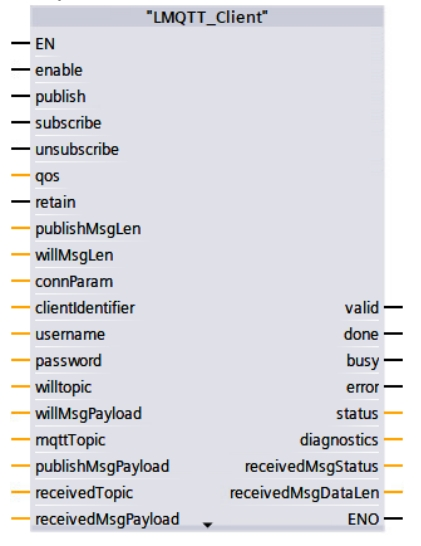
\includegraphics[width=0.6\textwidth]{images/LMQTT.jpeg}
	\caption{MQTT Funktionsblock im TIA Portal \autocite{siemensMQTT}}
	\label{fig:lmqtt}
\end{figure}

\section{Serial Peripheral Interface (SPI)}
\label{sec:spi}

Das \textbf{Serial Peripheral Interface (SPI)} ist ein synchrones serielles Kommunikationsprotokoll, das von Motorola in den 1980er-Jahren entwickelt wurde. Es wird häufig zur Kommunikation zwischen Mikrocontrollern und Peripheriegeräten wie Sensoren, Speicherchips oder Display-Treibern eingesetzt.

\subsection*{Grundprinzip}

SPI basiert auf einem \textit{Master-Slave}-Modell, bei dem der Master die Kommunikation initiiert und steuert. Ein oder mehrere Slaves reagieren auf die Befehle des Masters. Die Kommunikation erfolgt über vier Hauptleitungen:

\begin{itemize}
	\item \textbf{MOSI (Master Out Slave In)} – Datenleitung vom Master zum Slave
	\item \textbf{MISO (Master In Slave Out)} – Datenleitung vom Slave zum Master
	\item \textbf{SCLK (Serial Clock)} – Taktsignal, das vom Master bereitgestellt wird
	\item \textbf{SS / CS (Slave Select / Chip Select)} – Aktivierungssignal für einen spezifischen Slave (aktiv bei Low)
\end{itemize}

In \autoref{fig:spi3} wird die Funktionalität der Chip Select Leitung genauer beschrieben. Über SPI können mehrere Slaves mit einem Master verbunden werden, was eine gesteuerte Übertragung von Daten an einen ausgewählten Slave ermöglicht \autocite{mct_spi_2019}. Das geschieht mithilfe mehrerer Chip-Select-Leitungen am Master. Die serielle Datenleitung wird mit jedem Slave verbunden, durch Auswahl einer bestimmten Select-Leitung kann jedoch ausgewählt werden, an welchen Slave die Daten gerichtet sind. 

Die Serial-Data-Out-Leitungen können ebenso miteinander verbunden werden, da über die Select-Leitung bekannt ist, von welchem Slave die Daten kommen. Die Taktrate wird über das Serial-Clock-Signal vom Master vorgegeben. In dieser Arbeit ist jedoch nur eine SPI-Kommunikation mit einem Slave an jeweils einer Station relevant, weshalb pro Slave eine Select-Leitung in Snspruch genommen wird [siehe \autoref{sec:systementwurf}]. 

\begin{figure}[H] % [H] nur mit \usepackage{float}
	\centering
	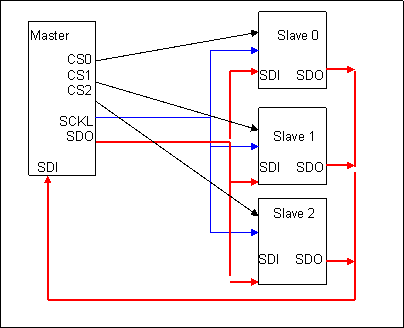
\includegraphics[width=0.8\textwidth]{images/spi3.png}
	\caption{Einzelnes Ansprechen der Slaves mittels Slave-Select-Leitungen (MOSI == SDO: Serial Data Out; MISO == SDI: Serial Data In) \autocite{mct_spi_2019}}
	\label{fig:spi3}
\end{figure}

\subsection*{Übertragungsmechanismus}

Die Kommunikation erfolgt bitweise synchron mit dem Taktsignal (SCLK). Bei jedem Taktzyklus wird ein Bit über MOSI (vom Master zum Slave) und gleichzeitig ein Bit über MISO (vom Slave zum Master) übertragen. Dadurch ist eine gleichzeitige (voll-duplex) Datenübertragung möglich.

Die SPI-Konfiguration wird durch vier Parameter definiert:
\begin{itemize}
	\item \textbf{Taktfrequenz} – Bestimmt die Geschwindigkeit der Datenübertragung
	\item \textbf{Datenrahmen} – Meist 8 Bit pro Übertragung
	\item \textbf{Bitreihenfolge} – MSB (Most Significant Bit) oder LSB (Least Significant Bit) zuerst
	\item \textbf{Clock Polarity und Phase (CPOL/CPHA)} – Steuert, bei welcher Flanke der Clock die Daten gelesen bzw. geschrieben werden
\end{itemize}
